\section{Resultados}
\subsection{Conversor digital-análogo}
\begin{figure}[H]
  \centering
  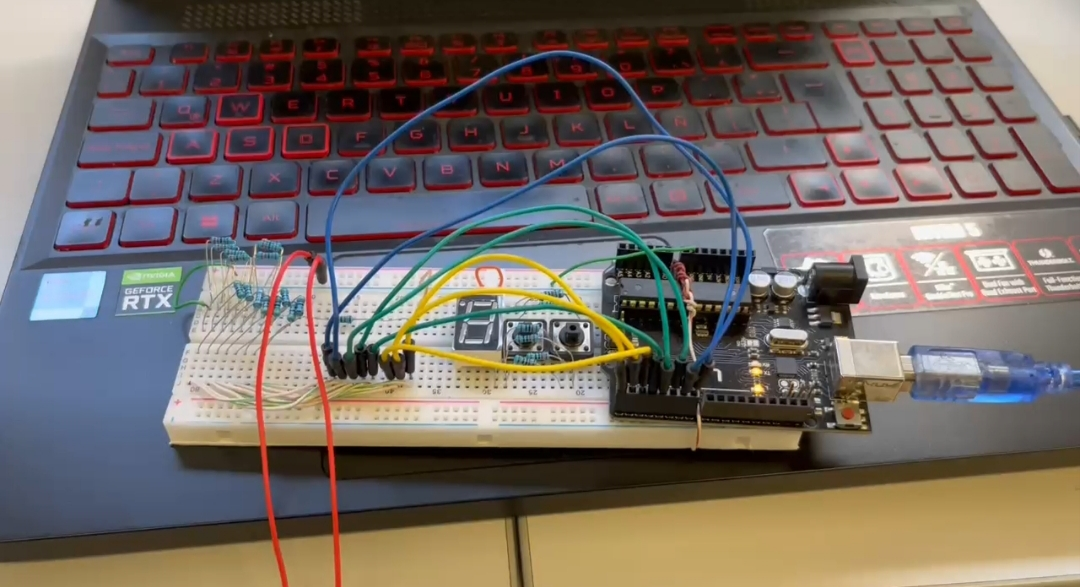
\includegraphics[width=\linewidth]{./Anexos/Resultados/DAC/Circuito.jpg}
  \caption{Circuito final para conversor digital-análogo. Fuente: \cite{LabDrive}.}
  \label{fig:conversor_circuito}
\end{figure}

\begin{figure}[H]
  \centering
  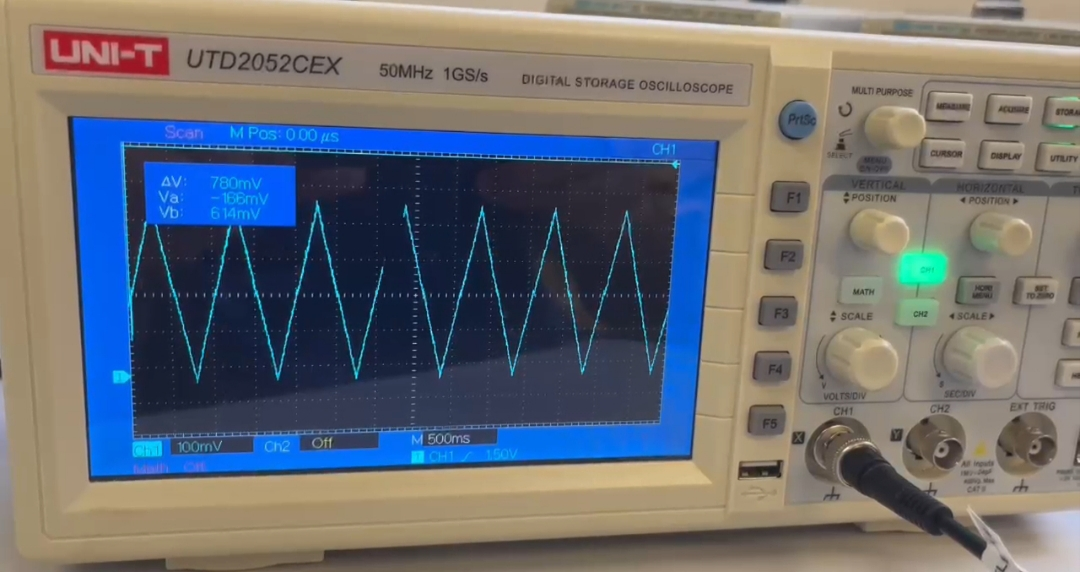
\includegraphics[width=\linewidth]{./Anexos/Resultados/DAC/Ocsiloscopio.jpg}
  \caption{visualización de señal en osciloscopio. Fuente: \cite{LabDrive}.}
  \label{fig:conversor_osciloscopio}
\end{figure}
\subsection{Matriz}

\subsubsection{Mapeado de puertos y pines}
Se mapean los puertos y pines individuales del mismo modo al que se puede apreciar en el anexo \ref{anexo:Look_Up_Table}.

\subsubsection{Encendido de un solo LED}
\begin{verbatim}
ldi ZH, high(ROW_PORTS<<1) 
ldi ZL, low(ROW_PORTS<<1)
add ZL, row adc ZH, r1  
lpm r16, Z ; r16 = row port adress
        
ldi ZH, high(ROW_MASKS<<1) 
ldi ZL, low(ROW_MASKS<<1)
add ZL, row adc ZH, r1
lpm r17, Z ; r18 = row pin mask

; Encender fila
clr ZH mov ZL, r16 
mov r16, r17
rcall CLEAR_BIT

ldi ZH, high(COL_PORTS<<1) 
ldi ZL, low(COL_PORTS<<1)  
add ZL, col adc ZH, r1  
lpm r16, Z ; r16 = column port adress

ldi ZH, high(COL_MASKS<<1) 
ldi ZL, low(COL_MASKS<<1)  
add ZL, col adc ZH, r1  
lpm r17, Z ; r17 = column pin mask

; Encender columna
clr ZH mov ZL, r16 
mov r16, r17
rcall SET_BIT
\end{verbatim}

\subsubsection{Multiplexado y dibujo de cuadros}
\begin{verbatim}
ldi row, 0 RENDER_FRAME_ROW_LOOP:  
ldi r16, 0b00000001 ; Frame mask
lpm r17, Z+

ldi col, 0 RENDER_FRAME_COL_LOOP:
    rcall CLEAR_MATRIX

    push r16
    and r16, r17

    cpi r16, 0 
    breq RENDER_FRAME_SKIP_LED

    rcall TURN_LED
    rcall TEST_DELAY

    RENDER_FRAME_SKIP_LED:
    pop r16
    lsl r16
inc col cpi col, 8 
brlo RENDER_FRAME_COL_LOOP 

inc row cpi row, 8 
brlo RENDER_FRAME_ROW_LOOP
\end{verbatim}

Manejo de cambio de estados utilizando USART para mostrar las diferentes imágenes en la matriz

\begin{verbatim}
USART_RX_ISR:	
    lds r16, UDR0

    ; Apagar pantalla
    cpi r16, '0' 
    breq USART_RX_ISR_CASE_0 

    ; Texto desplazante
    cpi r16, '1' 
    breq USART_RX_ISR_CASE_1 

    ; ...

USART_RX_ISR_CASE_0:
    rcall SET_ANIMATION_START
    ; Disable timer interrupts
    ldi r16, 0b0 sts TIMSK2, r16 
    ; Change state
    ldi r16, 0 mov current_state, r16   
    rjmp USART_RX_ISR_END

USART_RX_ISR_CASE_1:
    rcall SET_ANIMATION_START
    ; Change state
    ldi r16, 1 mov current_state, r16   
    ; Enable timer interrupts
    ldi r16, 0b1 sts TIMSK2, r16 
    rjmp USART_RX_ISR_END

    ; ...
\end{verbatim}

Aparte del manejo del cambio de estado, se implementó una máquina de estados, como la que se puede encontrar en el anexo \ref{anexo:Maquina_de_Estados}.

\begin{verbatim}
MAIN:
    rcall STATE_MACHINE
    rjmp MAIN
\end{verbatim}

\begin{figure}[H]
  \centering
  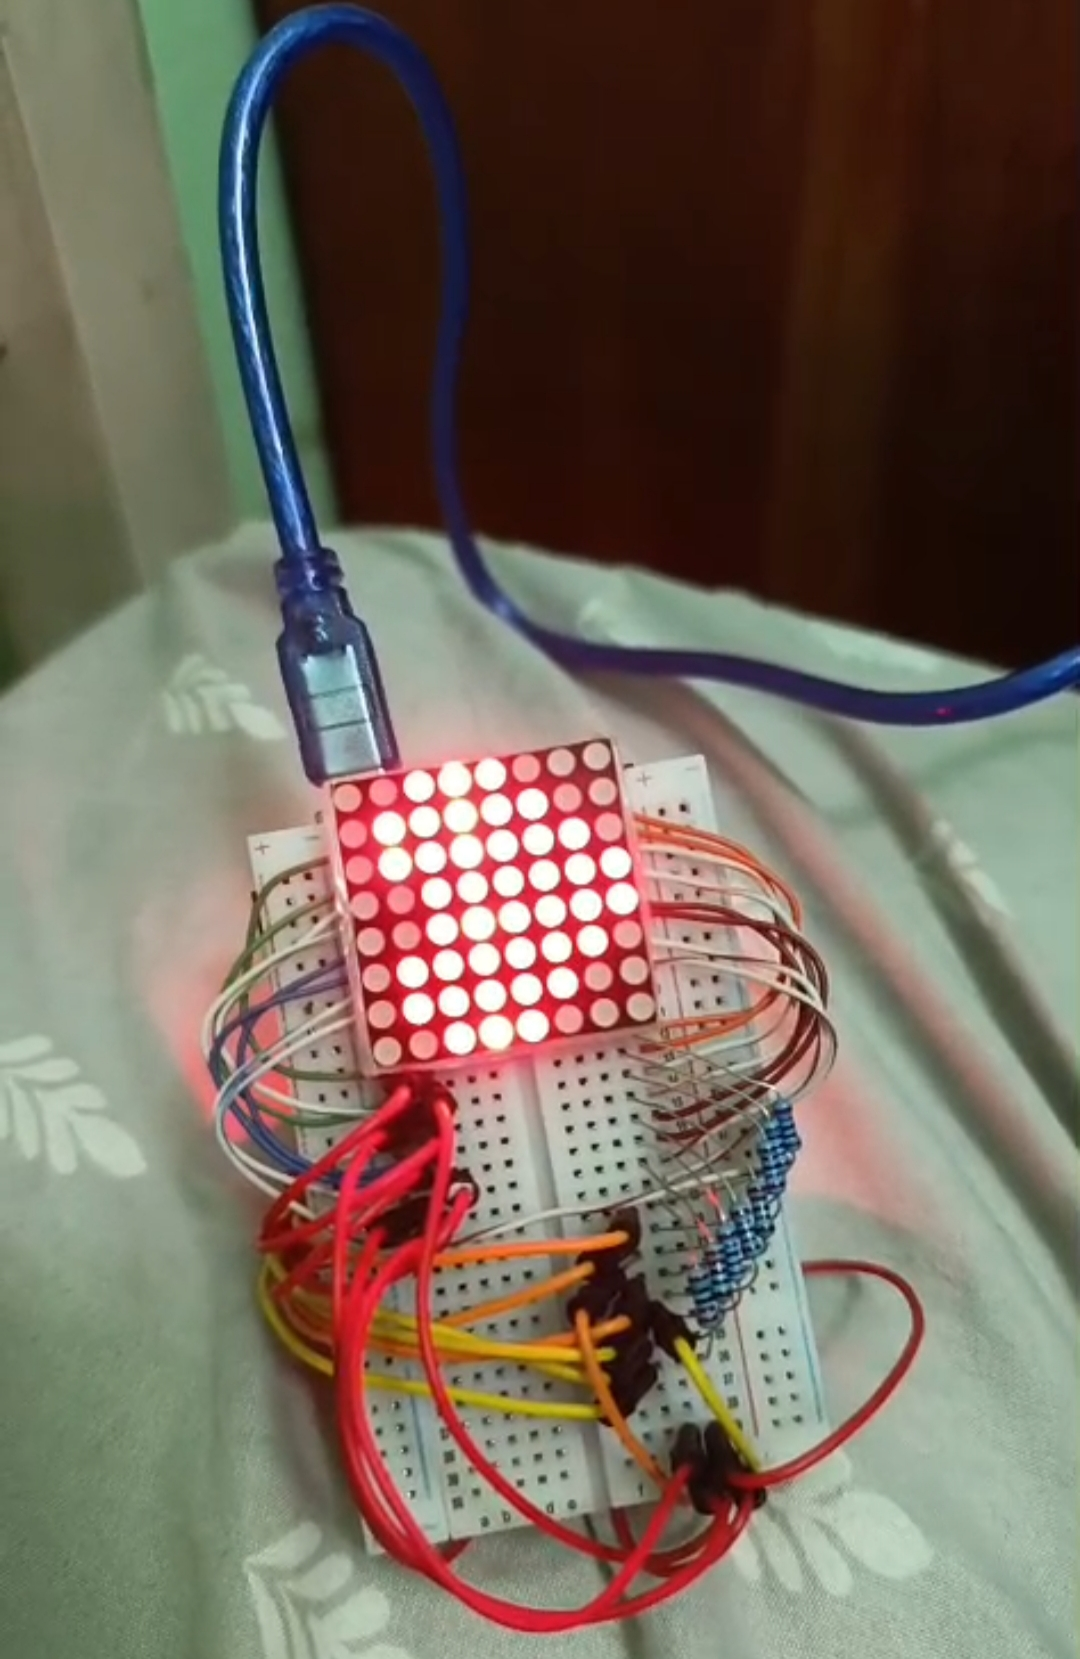
\includegraphics[width=0.7\linewidth]{./Anexos/Resultados/Matriz/Circuito.jpg}
  \caption{Circuito final para Matriz de LEDs. Fuente: \cite{LabDrive}.}
  \label{fig:circuito_matriz}
\end{figure}
\section{Punzonadora}

\begin{figure}[H]
  \centering
  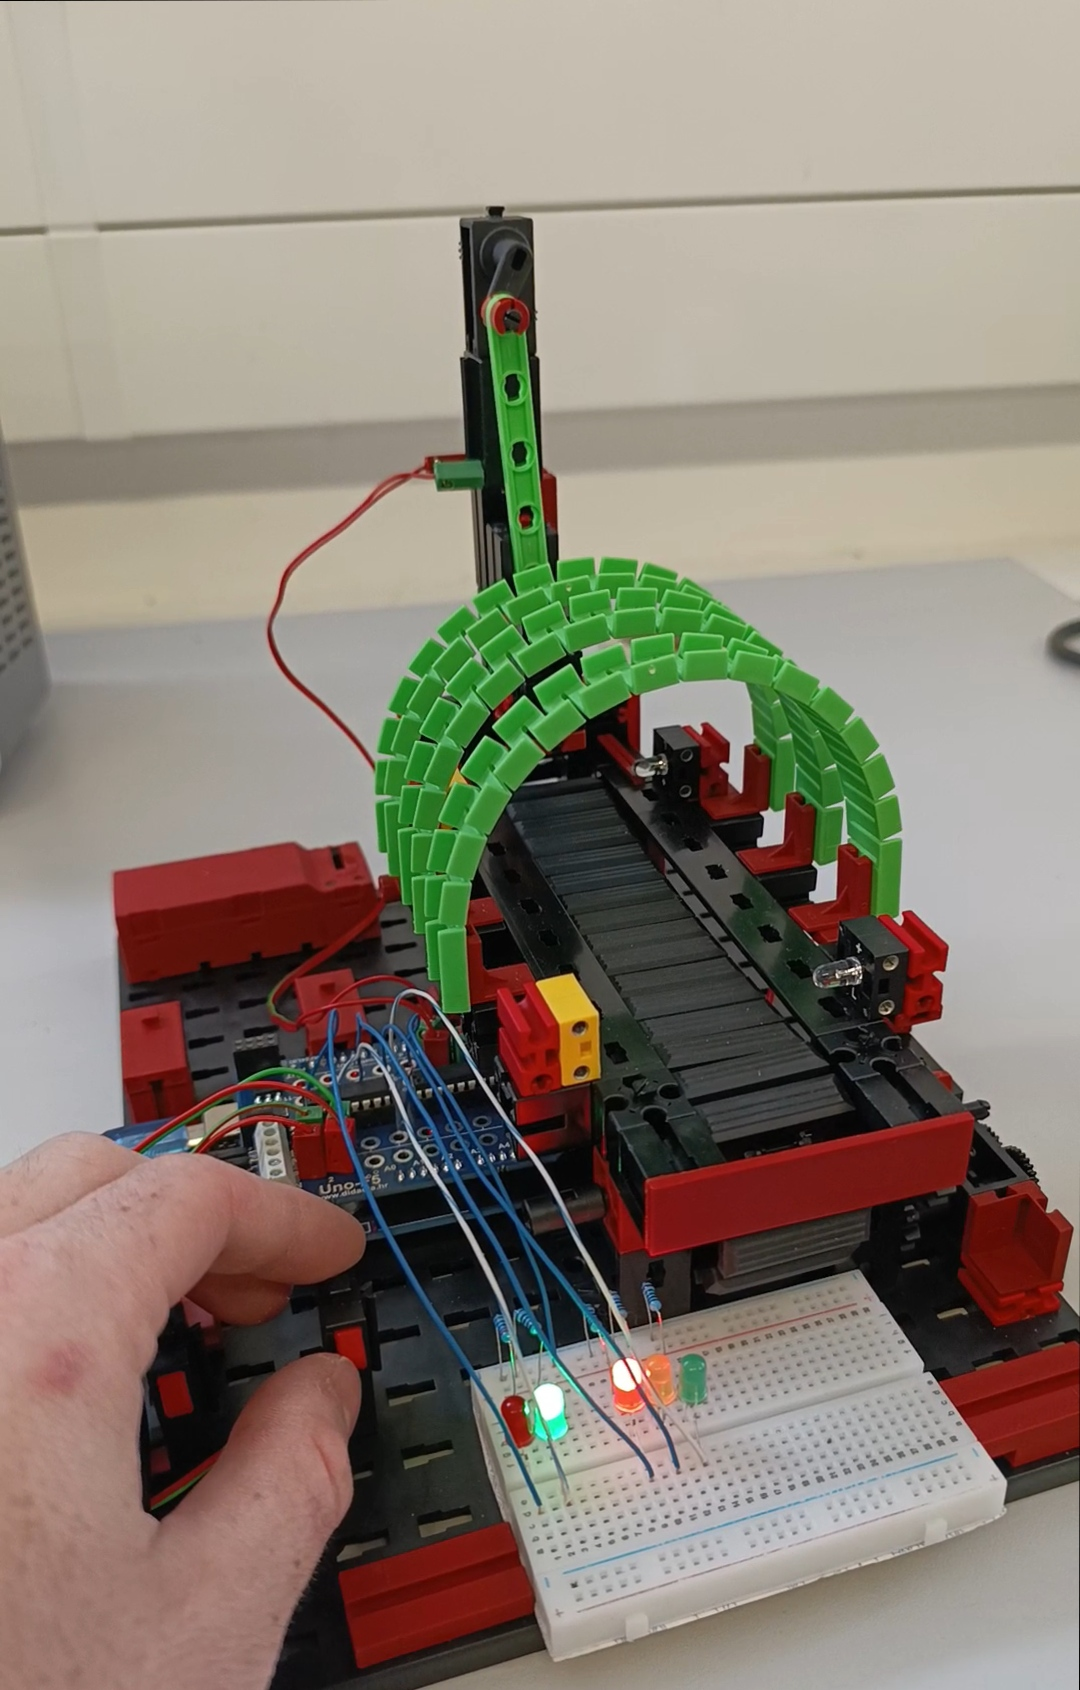
\includegraphics[width=0.7\linewidth]{./Anexos/Resultados/Punzonadora/Circuito.jpg}
  \caption{Ensamblado final de punzonadora. Fuente: \cite{LabDrive}.}
  \label{fig:punzonadora_circuito}
\end{figure}


\subsection{Plotter}
\begin{figure}[H]
  \centering
  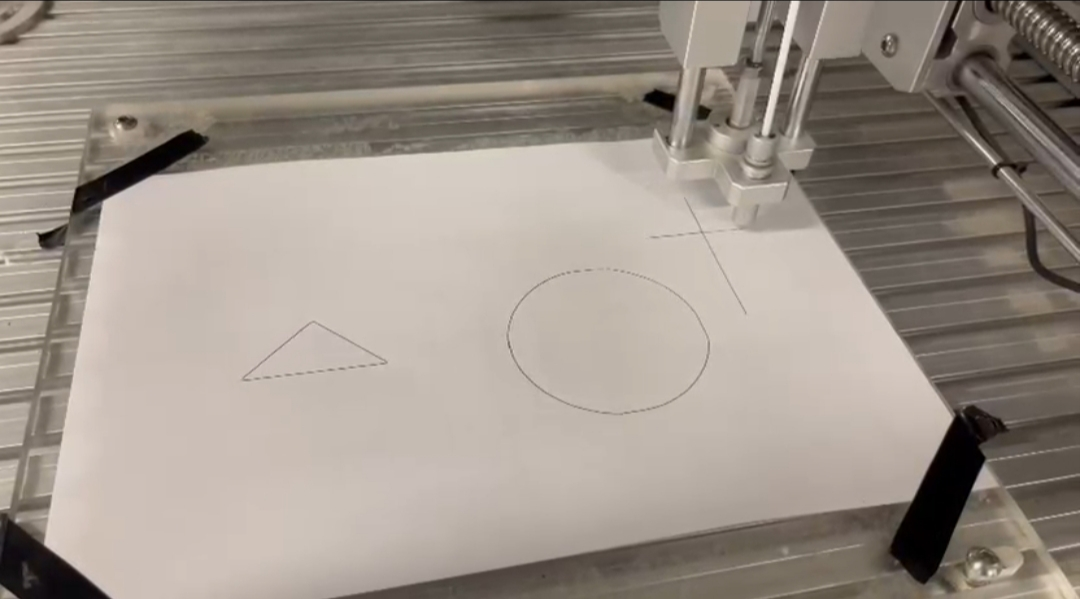
\includegraphics[width=\linewidth]{./Anexos/Resultados/Plotter/Dibujos.jpg}
  \caption{Figuras dibujadas en el plotter. Fuente: \cite{LabDrive}.}
  \label{fig:plotter_figuras}
\end{figure}